\vspace{-5pt}
\section{Benchmarking 
Retrieval Tasks over Textual and Relational Knowledge}
\vspace{-5pt}
% We develop three large-scale retrieval datasets on three semi-structured knowledge bases (SKBs) In Section~\ref{sec:def}, we introduce SKB and the problem setting.
% In Section~\ref{sec:skb}, we introduce the schema and scale of the SKBs, which integrate entities with rich relational and textual information. 
% In Section~\ref{sec:star}, we introduce the retrieval datasets and the key characteristics of the queries. Then, we highlight our novel dataset construction pipeline in Section~\ref{sec:construction}, which simulates user queries involving textual and relational knowledge and automatically generates the ground truth answers in the retrieval datasets.
% Finally, we conduct data distribution analysis and human evaluation on the queries in Section~\ref{sec:analysis}.
% % These knowledge bases integrate entities with detailed relational and textual information. 
% % Then the retrieval datasets are constructed in a way that assesses the model's proficiency in extracting information from varied data structures and synthesizing it to generate correct answers.

% \jure{You can cut this summary paragraph with forward references. It is a waste fo space}
% \jure{Instead you can have a section where you formally define the problem: We consider the following setting: SOMETHING LIKE THIS (PLEASE POLISH): We are given SKB, which is composed of a Knowledge Graph $G$ with a set of nodes and relations. We also assume that with each node $i$ there is a set of associated free text documents $D_i$. For example, in e-commerce, Knowledge Graph is a product knowledge graph capturing properties of products (brand, color) and the text documents correspond to reviews and product descriptions. Now given a Query $Q$, our goal is to find a set of answers that match the query. Answers are a subset of items in the knowledge graph. For example, in e-commerce answers are actual products.}


\begin{figure}[t]
    \centering
    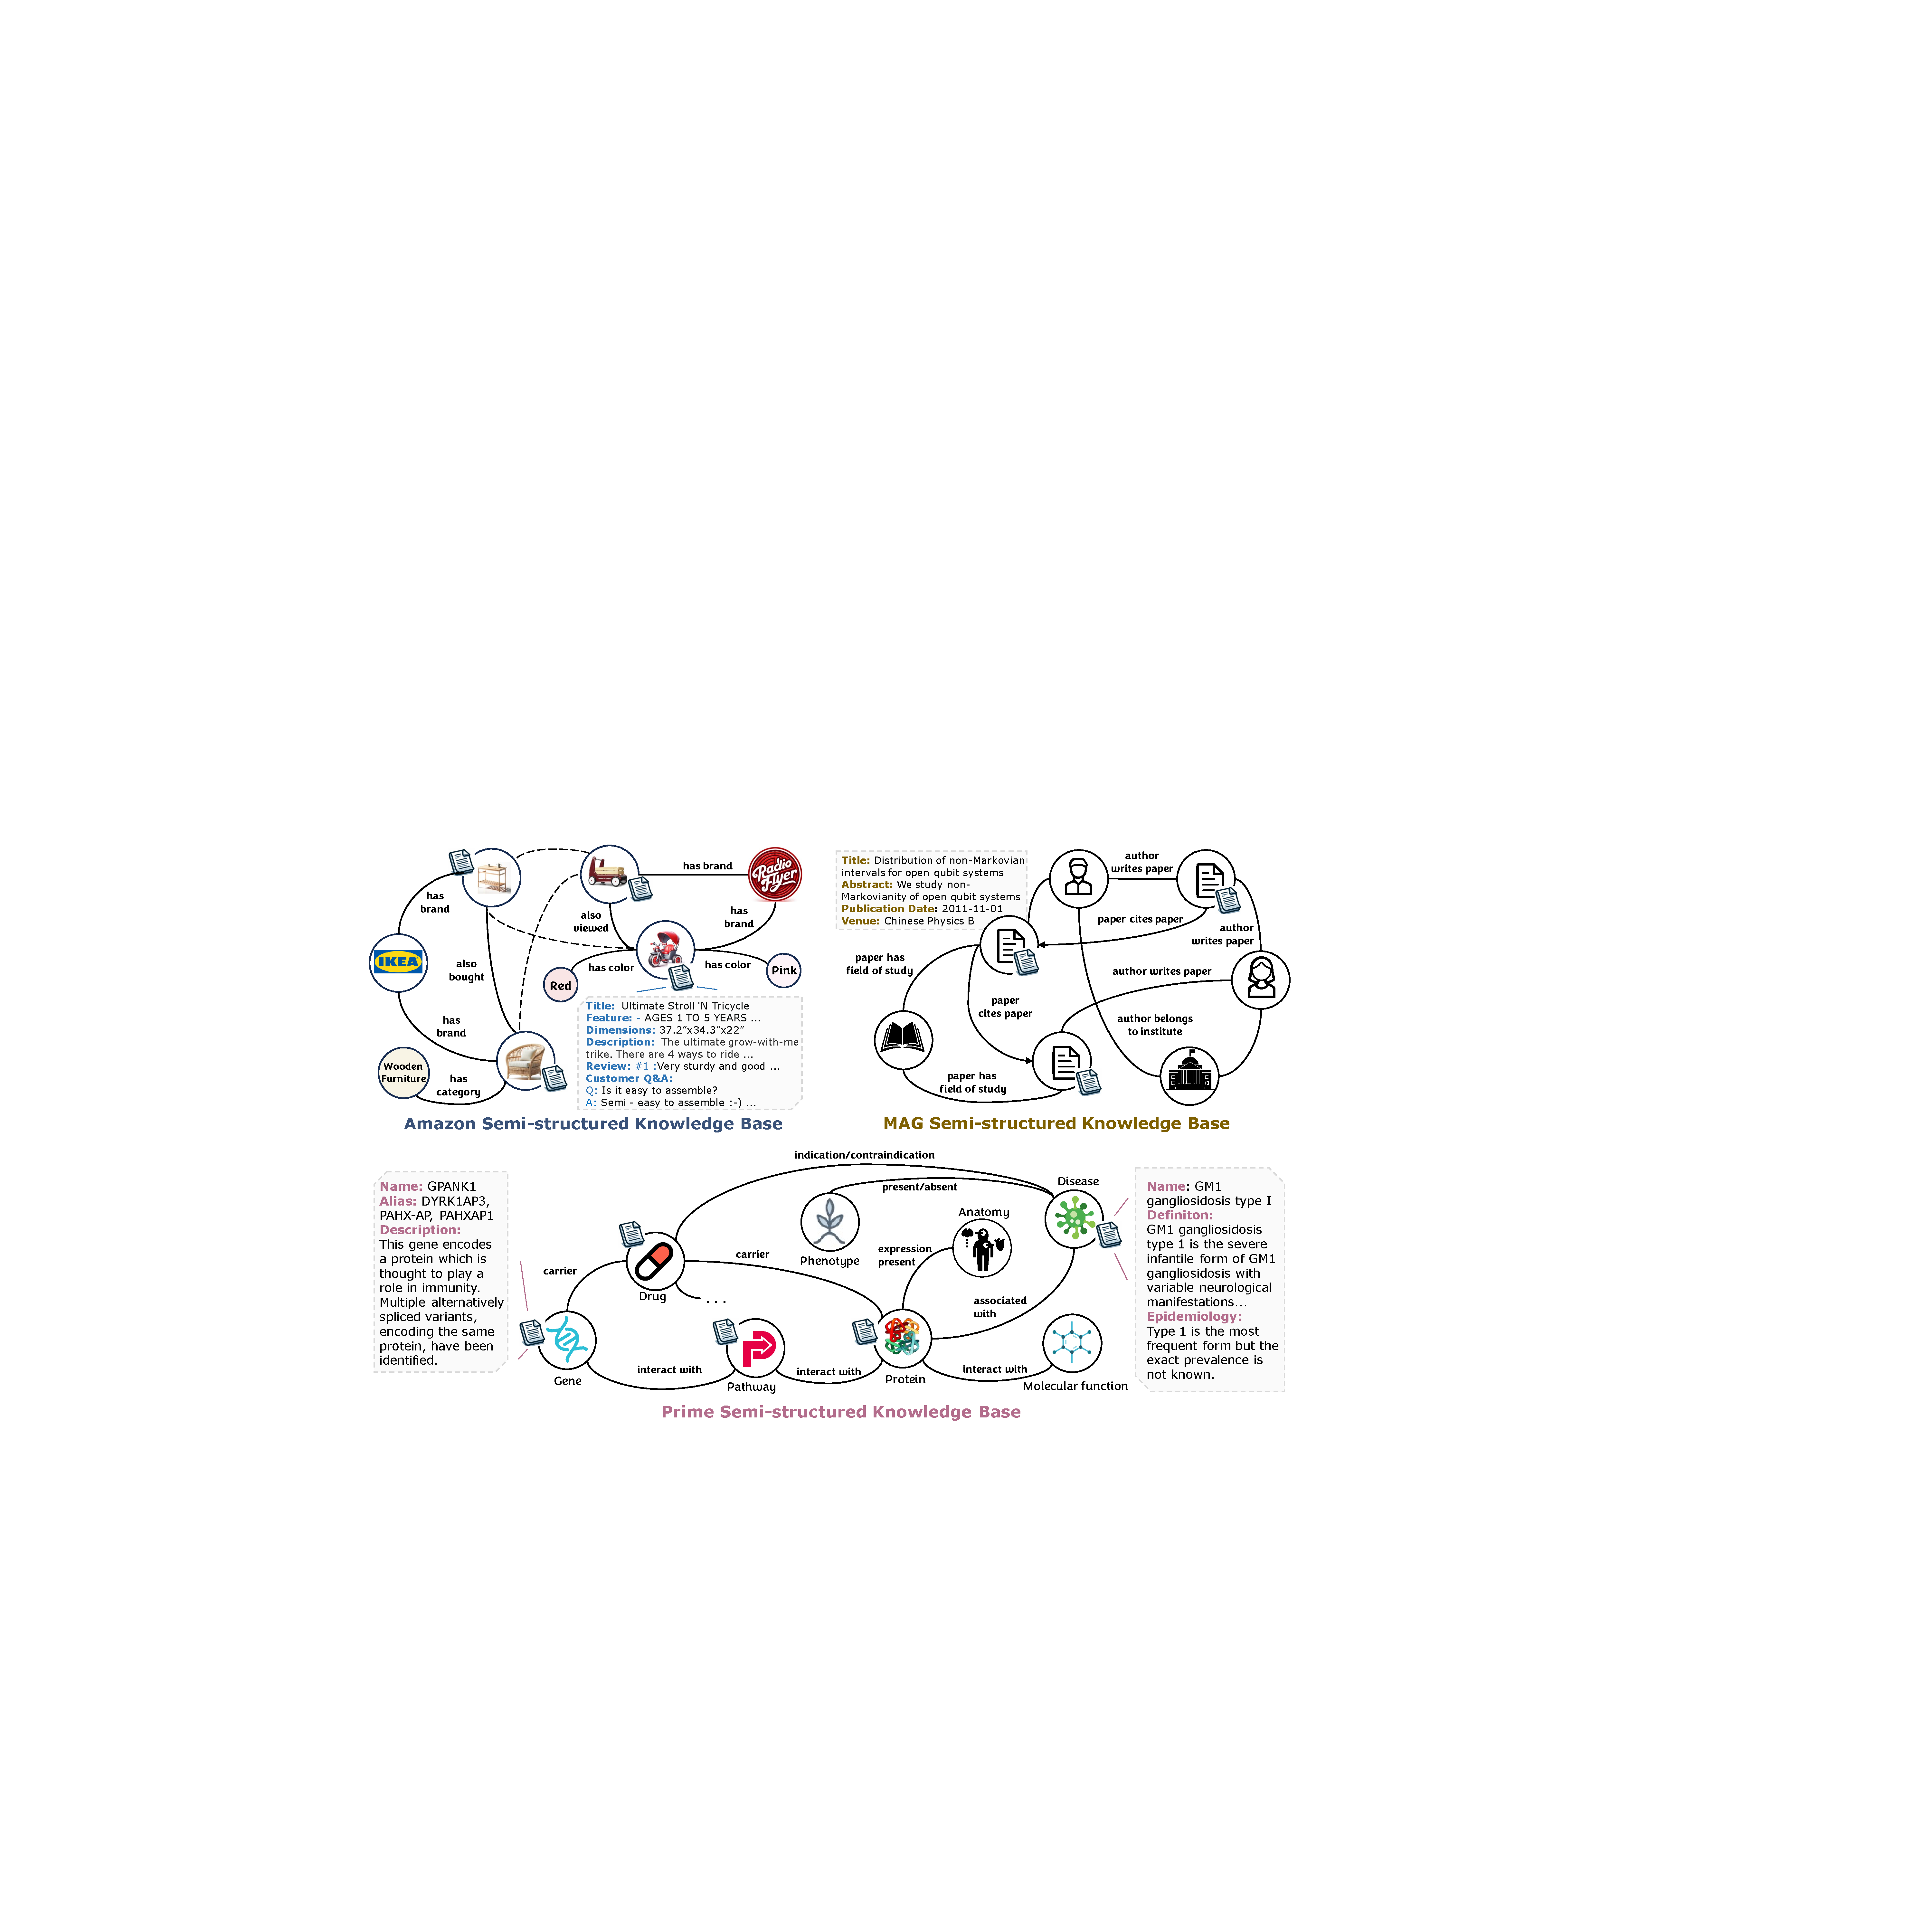
\includegraphics[width=0.98\textwidth]{figs/semistructure_v2}
    \vspace{-5pt}
    \caption{Demonstration of Semi-structured Knowledge Bases, 
    %\michi{You can also mention what you want readers to take away from this, e.g. "observe that semi-structured KB consists of text and relational info, which makes the task hard", etc.}
    where each knowledge base combines both textual and relational information in a complex way, making the retrieval tasks challenging.
    }
    \vspace{-15pt}
    \label{fig:semistructure}
\end{figure}

\subsection{\revision{Problem Definition}}
\label{sec:def}
\vspace{-3pt}
We are given a Semi-Structured Knowledge Base (SKB), which consists of a knowledge graph \( G \) and a collection of free text documents  $D$. 
% The knowledge graph \( G = (V, E) \) is composed of a set of nodes \( V \) and a set of edges \( E \), where each edge represents a relational link between nodes. Each node \( i \in V \) has an associated set of free text documents \( D_i \). 
Formally, let \( G = (V, E) \) be the knowledge graph, where \( V \) is the set of nodes and \( E \subseteq V \times V \) is the set of edges representing relationships between nodes. \( D = \bigcup_{i \in V} D_i \) be the collection of free-form text documents associated with the nodes, where \( D_i \) is the set of documents associated with node \( i \). For example, the product knowledge graph in e-commerce can capture relationships between products and brands/colors/categories, and the corresponding text documents include product descriptions, reviews, \etc

We define the tasks on our benchmark datasets as follows: 
Given the knowledge graph \( G = (V, E) \), a collection of free text documents \( D \), and a query \( Q \), the output is a set of nodes \( A \subseteq V \) such that for each node \( i \in A \), it satisfies the relational requirements imposed by the structure of \( G \) as specified in \( Q \), and the associated documents \( D_i \) satisfy the textual requirements specified in \( Q \). 

% v2: This work addresses semi-structured knowledge base retrieval, integrating relational and textual data extraction from databases \( \mathcal{D} = \{R, T\} \), with \( R \) and \( T \) representing relational and textual data, respectively. The objective is to construct a model \( f \) that, given a query \( Q = \{Q_r, Q_t\} \), maps it to an answer \( A \). The answer \( A \) are nodes in \( \mathcal{D} \) satisfying both relational \( Q_r \) and textual \( Q_t \) query parts. The task is defined as finding \( f: \{Q_r, Q_t\} \times \mathcal{D} \rightarrow A \), effectively merging \( R \) and \( T \) to generate \( A \). The input of the model is semi-structure knowledge base and a query, and the output should be a set of predicted answers.

\vspace{-3pt}
\subsection{Semi-structured Knowledge Bases (SKBs)}
\label{sec:skb}
\vspace{-3pt}

\begin{table}[t]
    \centering
    \caption{Data statistics of our constructed semi-structured knowledge bases}
    \resizebox{0.92\textwidth}{!}{
    \begin{tabular}{l|ccrrrr}
        \toprule
        \multirow{ 2}{*}{} & \textbf{\#entity} & \textbf{\#relation} & \textbf{avg. } & \multirow{ 2}{*}{\textbf{\#entities}} & \multirow{ 2}{*}{\textbf{\#relations}} & \multirow{ 2}{*}{\textbf{\#tokens}} \\
        & \textbf{types} &\textbf{types} & \textbf{degree}\\
        \midrule
        \amazont & 4 & 5  & 18.2 & 1,035,542 & 9,443,802 & 592,067,882\\
        \magt & 4 & 4  & 43.5& 1,872,968 & 39,802,116 & 212,602,571\\
        \primekgt & 10& 18 & 125.2 & 129,375 & 8,100,498  & 31,844,769\\
        \bottomrule
    \end{tabular}
    }
    \vspace{-15pt}
    \label{tab:statistics}
\end{table}

As shown Figure~\ref{fig:semistructure}, we construct three large-scale SKBs with the relational and textual information with each entity. 
See Table~\ref{tab:statistics} for the basic data statistics and Appendix~\ref{app:skb} for details.
% \karthik{Refer this table at the end of this section along with other Appendices. Seems out of place.}
% See Table~\ref{tab:sources} for the comprehensive public sources we used to construct the SKBs. 

\xhdr{Amazon Semi-structured Knowledge Base}  
The SKB features four entity types: \texttt{product}, \texttt{brand}, \texttt{color}, and \texttt{category}, and five relation types:  \texttt{also\_bought, also\_viewed} between \texttt{product} entities, and
\texttt{has\_brand/color/category} associated with the products. 
We derive the textual information of \texttt{product} nodes by combining Amazon Product Reviews~\cite{ups-amazon_review} with Amazon Q\&A Data~\cite{image_amazon_qa}. 
This provides a rich amount of texts, including product descriptions and customer reviews. 
For other entities, we extract their names or titles as the textual attributes. Amazon SKB features an extensive textual data largely contributed from customer reviews and Q\&A.

\xhdr{MAG Semi-structured Knowledge Base} 
This SKB includes node entities of \texttt{paper}, \texttt{author}, \texttt{institute}, and \texttt{field\_of\_study}. We derive its relational structure by extracting a subgraph from obgn-mag~\cite{hu2021open}, which contains shared paper nodes with obgn-papers100M~\cite{hu2021open} and all non-paper nodes. We filter out non-English language papers as we only consider single-lingual queries. 
The paper documents include their titles and abstracts. Additionally, we integrating details from the Microsoft Academic Graph database (version 2019-03-22)~\cite{mag, mag_data}, providing extra textual information like paper venue, author and institution names. 
This SKB demonstrates a large number of relations associate with \texttt{paper} nodes, especially on citation and authorship relations. 


\xhdr{Prime Semi-structured Knowledge Base} We leverage the exisiting knowledge graph PrimeKG~\cite{primekg} which contains ten entity types including \texttt{disease, gene/protein}, and eighteen relation types, such as \texttt{associated\_with, indication}.
Compared to the Amazon and MAG SKBs, Prime SKB is denser and features a greater variety of relation types. While PrimeKG provides text information on \texttt{disease} and \texttt{drug} entities, 
% including drug mechanisms and disease descriptions, 
we integrate the data from multiple databases for \texttt{gene/protein} and \texttt{pathway} entities such as genomic position, gene activity summary and pathway orthologous event.





\subsection{Retrieval Tasks on Semi-structured Knowledge Bases}
\label{sec:star}
Our retrieval benchmark (Table~\ref{tab:benchmark_stats}) consists of three novel retrieval-based question-answering datasets, each comprising synthesized train/val/test sets with $9$k to $14$k queries in total and a high-quality human-generate query set.
% Specifically, the task is to retrieve items  over the SKBs given any input queries. 
The queries synthesize relational and textual knowledge, mirroring real-world queries in terms of natural-sounding property and flexible formats.

% Our retrieval benchmark, detailed in Table~\ref{tab:benchmark_stats}, comprises between $9$k to $14$k queries per dataset. Below, we outline the task on each dataset:

% Each query may have single answer or multiple answers, formulated as a subset of entities \revision{in the knowledge graph,}
% \jure{This is wrong. Entities are in the knowlede graph, Knowledge Base contains documents as well but those are not answers}
% which requires the model to accurately identify the ground truth entities out of potentially millions in response to each query.
% In Table~\ref{tab:benchmark_examples}, we demonstrate example queries from these benchmarks. 
\xhdr{\amazont} 
% This dataset comprises 9,100 synthesized customer-focused queries \hw{along with 81 human-generated queries for additional evaluation}. 
The task aims at product recommendation, with a notable 68\% of the synthesized queries yielding more than one ground truth answer. The dataset prioritizes customer-oriented criteria, highlighting textual elements such as product quality, functionality, and style. Moreover, it incorporate single-hop relational aspects (Appendix~\ref{app:amazon}) into the queries, including brand, category, and product connections (\eg complementary or substitute items). The queries are framed in conversation-like formats, enriching the context and enhancing the dataset's relevance to real-world scenarios.


% true positive: 86.6\%
% true negative: 96.7\%
\xhdr{\magt} 
% This dataset comprises 13,323 synthesized \hw{and 84 human-generated queries targeting at academic paper search.} 
Beyond the single-hop relational requirements in \amazont, \magh emphasizes the fusion between the textual requirements with multi-hop queries for precise academic paper search. For example, ``Are there any papers from King's College London'' highlights the metapath (\texttt{institution $\rightarrow$ author $\rightarrow$ paper}) on the relational structure. 
We designed three single-hop and four multi-hop relational query templates (Appendix~\ref{app:mag}). The textual aspects focus on the paper's topic, methodology, and contribution \etc
% true positive: 98.9\%

\xhdr{\primekgt} 
% This dataset, comprising 11,204 synthesized queries and \hw{109 human-generated queries across all ten entity types,} incorporates single-hop and multi-hop relational information similar to \magt. 
% For synthesized queries, we developed 28 multi-hop query templates, detailed in Appendix~\ref{app:prime}, to cover various relation types and ensure their practical relevance. 
% For instance, the query ``What is the drug that targets the genes or proteins expressed in <anatomy>?'' serves applications in precision medicine and pharmacogenomics, 
% aiding researchers and healthcare professionals in identifying drugs that act on genes or proteins associated with specific anatomical areas and enabling more targeted treatments. 
The task is to answer complex biomedicine inquiries. 
For synthesized queries, we developed 28 multi-hop query templates (Appendix~\ref{app:prime}) to cover various relation types and ensure their practical relevance. 
For example, the template ``What is the drug that targets genes or proteins in <anatomy>?'' aids precision medicine by identifying treatments targeted to specific anatomical areas.
For \texttt{drug, disease, gene/protein}, and \texttt{pathway} entities, the queries are a hybrid of relational and textual requirements. 
For entities such as \texttt{effect/phenotype}, the queries rely solely on relational data due to limited textual information. 
We exhibit three distinct user roles – medical scientist, doctor, and patient – for generating queries about drug and disease, which diversify the language to comprehensively evaluate the retrieval systems.



\begin{table}[t]
    \centering
    \caption{Statistics on the \benchmarkh benchmark datasets.}
    \resizebox{0.9\textwidth}{!}{
    \begin{tabular}{ll|rrrr}
        \toprule
        & & \multirow{2}{*}{\textbf{ \#queries}}  & \textbf{ \#queries w/} & \textbf{average} & \multirow{2}{*}{\textbf{train / val / test}}\\
        & & & \textbf{multiple answers}&  \textbf{\#answers} & \\
        \midrule
        \multirow{3}{*}{
        \makecell{Synthesized\\
        (Sec~\ref{sec:construction}, \ref{sec:analysis})}} & {\small \amazont} & 9,100 & 7,082  & 17.99& {0.65 / 0.17 / 0.18}\\
        & {\small \magt} &13,323 & 6,872 & 2.78 & {0.60 / 0.20 / 0.20}\\
        & {\small \primekgt} & 11,204 & 4,188 & 2.56 & {0.55 / 0.20 / 0.25} \\
        \midrule
        \multirow{3}{*}{\makecell{Human-generated\\
        (Sec~\ref{sec:human_generated})}} 
        & {\small \amazont} & 81 & 64 & 19.50 & \multirow{3}{*}{For testing only}\\
        & {\small \magt} & 84 &34 & 3.26 & \\
        & {\small \primekgt} & 98 & 41 & 2.77 & \\
        \bottomrule
        \end{tabular}
        }
    \vspace{-5pt}
    \label{tab:benchmark_stats}
\end{table}
\begin{figure}[t]
    \centering
    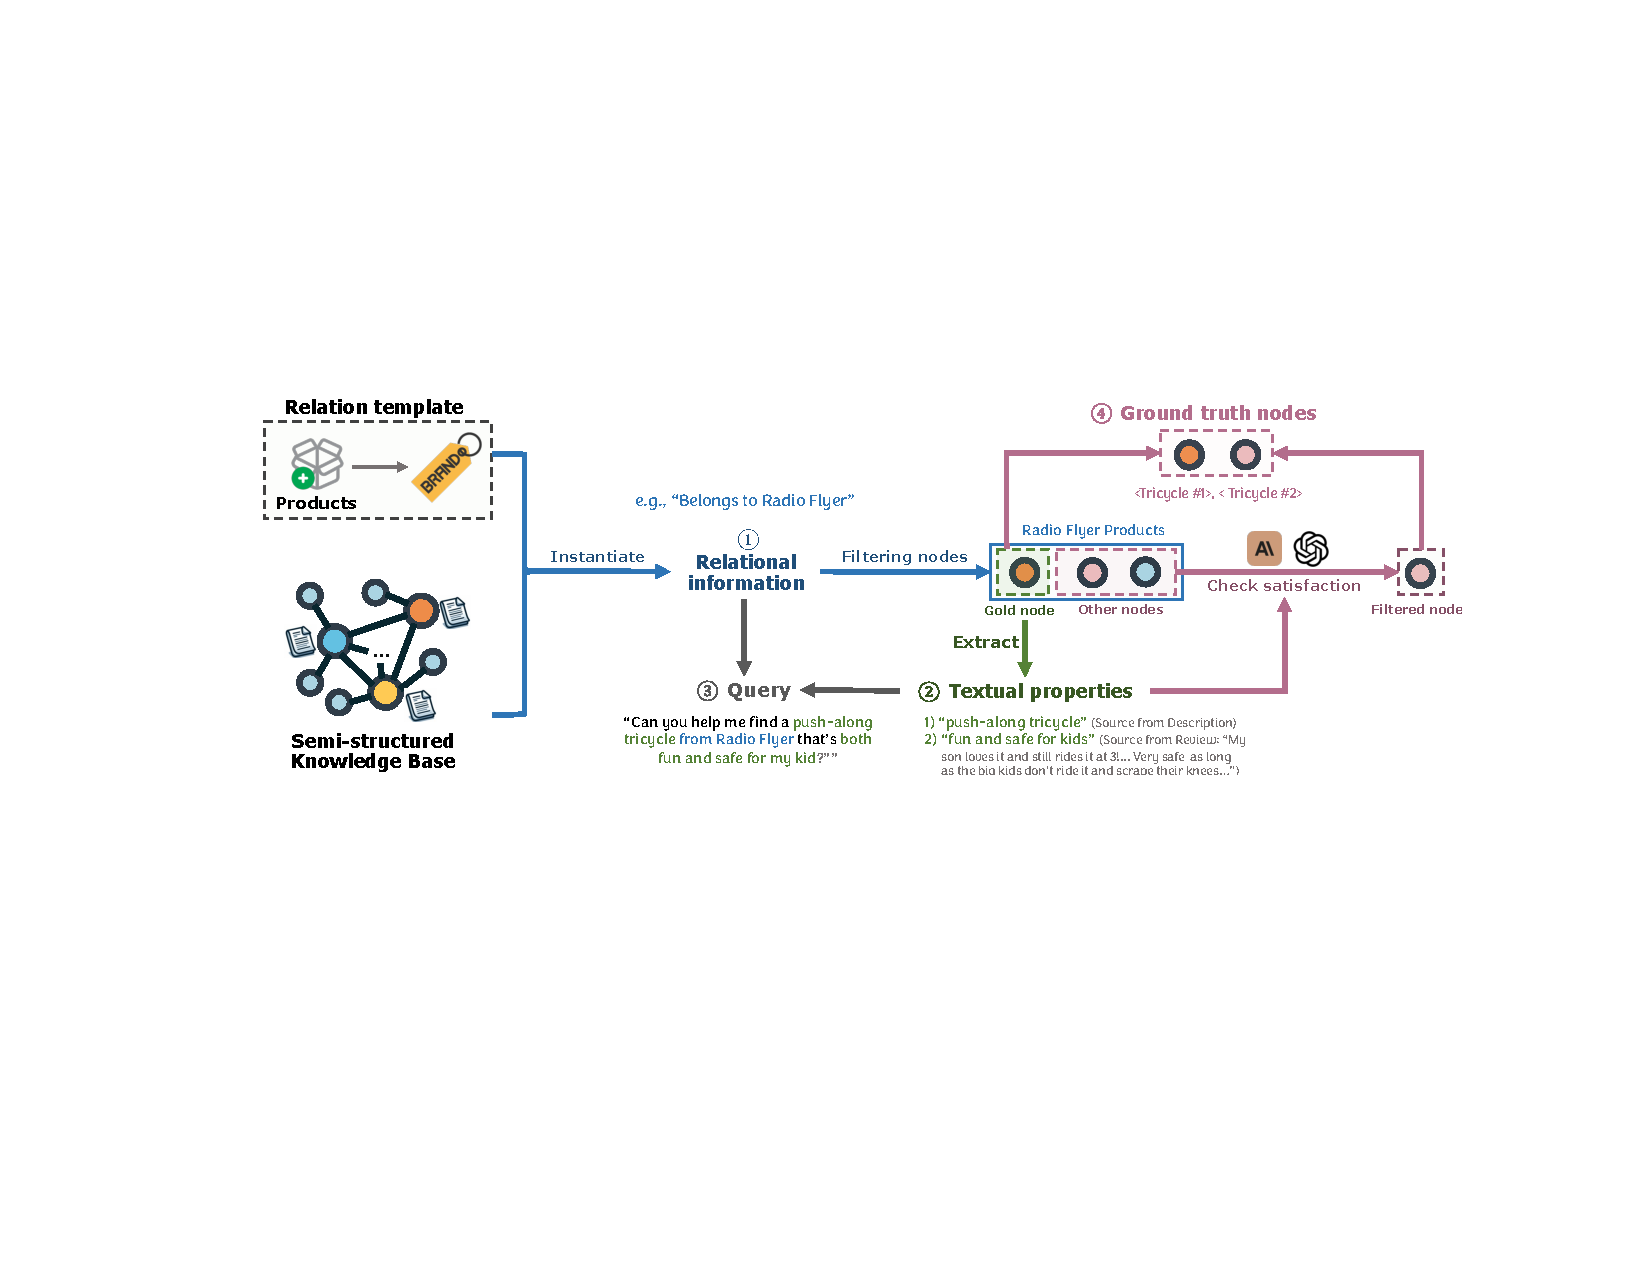
\includegraphics[width=0.95\textwidth]{figs/construction}
    \vspace{-3pt}
    \caption{
    The construct pipeline to generate our semi-structured retrieval datasets.
    % involves four main steps: 1) Sample Relational Requirement: Based on relational templates, sample a relational requirement on a SKB.
    % 2) Extract Textual Properties: From a node that meets the relational requirement, extract relevant textual properties.
    % 3) Combine Information: Merge the relational information and textual properties to form a natural-sounding query.
    % 4) Construct Ground Truth Nodes: Check if nodes satisfy the textual properties using multiple language models to establish ground truth nodes.
    }
    \vspace{-10pt}
    %\kexin{what is the meaning of edge color?}
    %\shirley{the edge colors are made the same as the arrow color}
    \label{fig:construction}
\end{figure}

\vspace{-2pt}
\subsection{Benchmark Construction: Synthesized Queries} 
\label{sec:construction}
\vspace{-2pt}
% \karthik{this section needs a running example and should be tied closely to the numbering in Fig 5}
In Figure~\ref{fig:construction}, we present a novel pipeline that synthesizes the SKB queries and automatically generates the ground truth answers. 
The key idea is to entangle relational and textual information during synthesis and disentangle them during answer filtering. 
It involves four steps as follows:
% The pipeline involves four steps and the specific processes vary depending on the characteristics of each dataset. These steps are as follows:

% We leverage the GPT and Claude language models to construct the retrieval datasets. Detailed descriptions of all the prompts we used are available in Appendix~\ref{app:prompts}. 

\begin{itemize}[leftmargin=*]
\vspace{-2pt}
\item \textbf{1) Sample Relational Requirements:} For each query, we sample a practical relation template constructed with expert/domain knowledge, \eg ``\texttt{(a product) belongs to <brand>}'' and ground it with sampled entities (\ie a specific brand), \eg ``belongs to Radio Flyer''. 
This relational requirement yields a set of candidate entities, \ie products belonging to Radio Flyer. 
% \revision{The relation templates for the three SKBs are practical and constructed with expert/domain knowledge}, which are available in Appendix~\ref{app:details}. 
% Therefore, we obtain the relational requirements and the corresponding candidates. 
% For instance, the template ``What is the drug that targets the genes or proteins which are expressed in <anatomy>?'' is particularly valuable for precision medicine inquiries. It aids in pinpointing medications aimed at specific genetic or protein targets within defined anatomical areas, thereby contributing to the development of targeted treatments. 
% \shirley{relate text to figure, \eg step 1}
\vspace{-2pt}
\item \textbf{2) Extracting Textual Properties:} \revision{
% The relational requirement yields a set of satisfying candidates. 
We randomly sample a candidate entity from the first step, referred to as the \textit{gold answer}, from which LLMs extract properties that align with the interests of specific roles (\eg customers, researchers, or doctors) in its textual document}.  In Figure~\ref{fig:construction}, we extract multiple properties about the functionality and user experience from a Radio Flyer product. 
%%%%%% We utilize GPT-3.5-turbo-16k for the \amazonh and Claude-v2 for the other two datasets to conduct this step, where the prompts used are included in Appendix~\ref{app:prompts}.  
% \karthik{how?}
\vspace{-2pt}
\item \textbf{3) Combining Textual and Relational Information:} 
We use two LLMs to synthesize queries from textual properties and relational requirements, enhancing diversity and reducing bias arise from relying on a single LLM. 
The first LLM focuses on generating natural, role-specific, and style-consistent (\eg ArXiv searches) queries. The second LLM enriches the context and rephrases queries, which poses the need for advanced reasoning to comprehend them under complex contexts.

\vspace{-2pt}
\item \textbf{4) Filtering Additional Answers:} 
Finally, we employ multiple LLMs to verify if the candidates from the first step meet the extracted textual properties. Only candidates passing all LLM verifications are included in the final ground truth set. To assess the precision of this filtering mechanism, we compute the average ratios for the gold answers to be verified, which are 86.6\%, 98.9\%, and 92.3\% on the three datasets, highlighting our efficacy in yielding high-quality ground truth answers.

\vspace{-2pt}
\end{itemize}

This dataset construction pipeline is automatic, efficient, and broadly applicable to the SKBs in our formulation.  
\revision{We include all of the prompts and the LLMs versions in the above steps in Appendix~\ref{app:prompts}.} 



\begin{figure}[t]
    \centering
    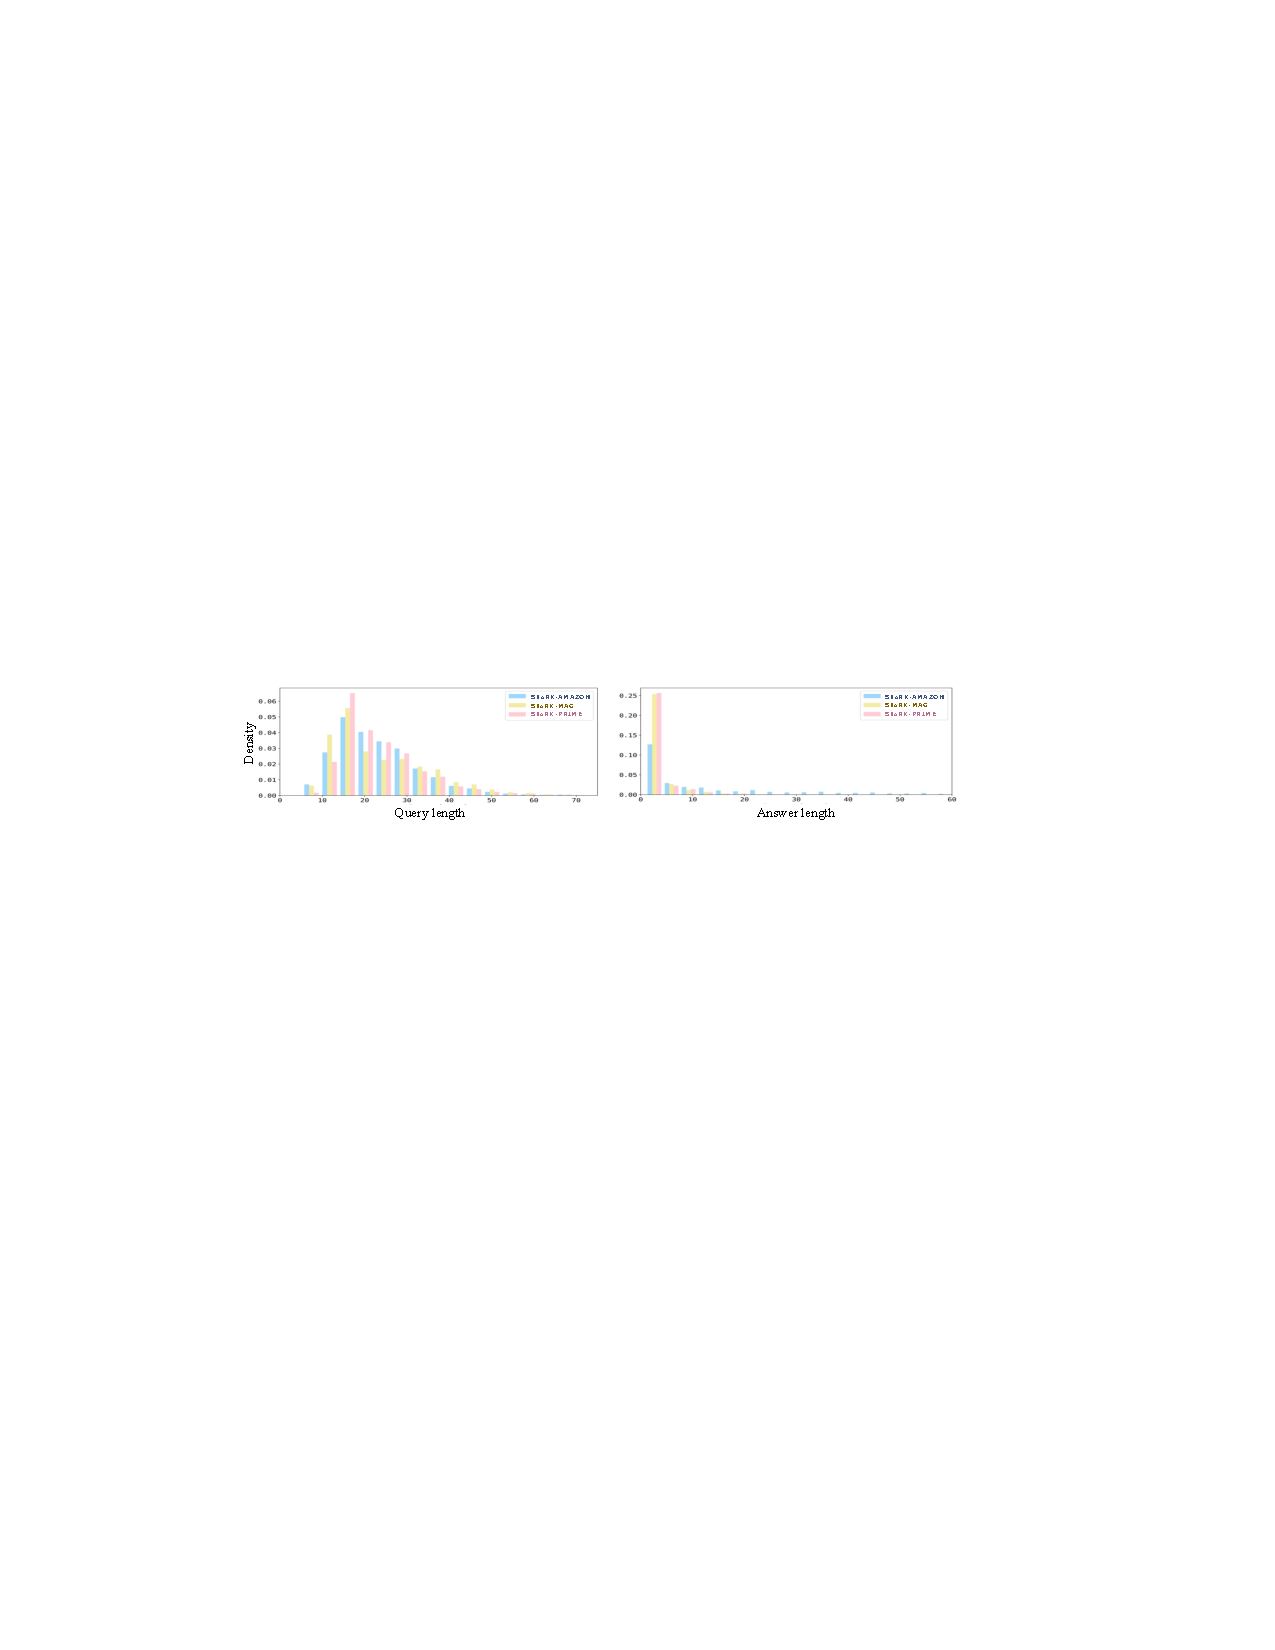
\includegraphics[width=1\textwidth]{figs/length_histv2}
    \vspace{-15pt}
    \caption{Distribution of query and answer lengths on \benchmarkh datasets.}
    \vspace{-5pt}
    \label{fig:length_dist}
\end{figure}

\begin{figure}[t]
    \begin{minipage}[t]{0.5\textwidth}
        \centering
      \captionof{table}{Query diversity measurement on \benchmarkt. \revision{See Appendix~\ref{app:math} for the metric definition.}}
      \vspace{5pt}
        \resizebox{1\textwidth}{!}{
        \begin{tabular}{l|cc}
            \toprule
            & {\small Shannon Entropy} & {\small Type-Token Ratio} \\
            % & {\small Entropy} & {\small Ratio} \\
            \midrule
            \small \amazonh & 10.39 & 0.179 \\
            \small \magh & 10.25 & 0.180 \\
            \small \primekgh & 9.63 & 0.143 \\
            \midrule
            \small Reference article & 10.44 & 0.261\\
            \bottomrule
        \end{tabular}
        }
        \label{tab:q_diversity}
    \end{minipage}%
    \hfill 
    \begin{minipage}[t]{0.47\textwidth}
        \caption{Average relative composition of relational vs. textual information.}
        \vspace{-5pt}
        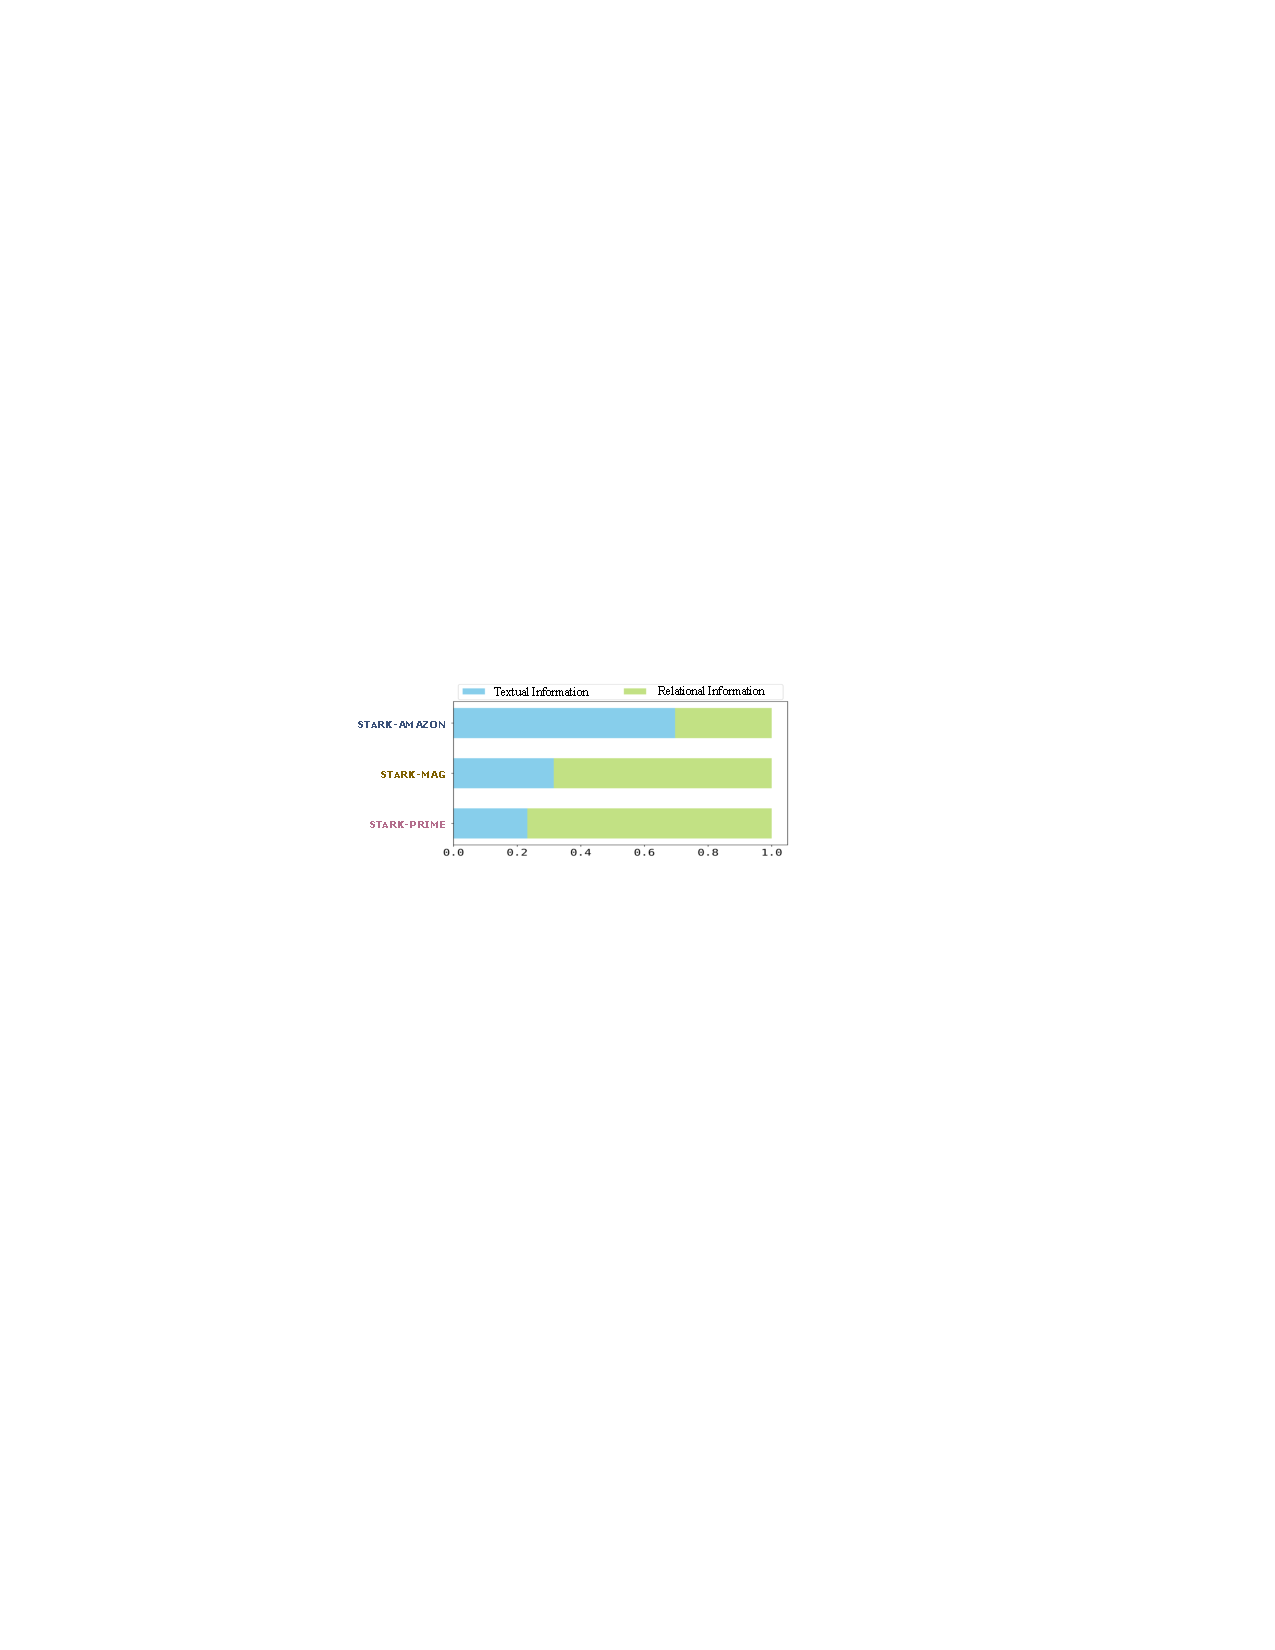
\includegraphics[width=\textwidth]{figs/ratiov2}
        \label{fig:ratio}
    \end{minipage}
    \vspace{-20pt}
\end{figure}


\subsection{Synthesized Data Distribution Analysis and Human Evaluation}
\label{sec:analysis}


% We conduct analysis and human evaluation on our synthesized datasets across three dimensions.
% to understand their characteristics and assess benchmark quality through human evaluation.
\begin{itemize}[leftmargin=*]
    \item \xhdr{Query and Answer Length} 
    Query length (in words) reflects the amount of user-provided context information, while the number of answers indicates query ambiguity/concreteness.
    Figure~\ref{fig:length_dist} shows similar query length distributions across the datasets, with most queries around 16 words. Longer queries (up to 50 words) often mention other entities or provide detailed context. Notably, 
    \amazonh has a significant long-tail pattern, with about 22\% of the answers have more than 30 entities, reflecting diverse e-commerce recommendations and ambiguous user queries.
    % , which results in a higher average answer length in 
    % Table~\ref{tab:benchmark_stats}
     
    \item \xhdr{Query Diversity} %  and Answer Coverage
    A diverse set of queries poses challenges for broader applicability to meet varying user demands. We measure query diversity using Shannon Entropy for word distribution and Type-Token Ratio (TTR) for unique words. Higher values indicate greater lexical diversity. Table~\ref{tab:q_diversity} shows high Shannon Entropy and steady TTR across all datasets. For reference, we compute these metrics for the Wikipedia page of Barack Obama\footnote{\url{https://en.wikipedia.org/wiki/Barack\_Obama}}. 
    
    \item \xhdr{Proportionality of Relational \textit{vs.}Textual Information}
    Our benchmark queries feature the composition of textual and relational information. To understand the distribution of information types, we calculate the average ratio of relational to textual requirements by word count in the queries across each dataset.  
    Note that the ratios do not directly reflect their importance in determining final answers. Figure~\ref{fig:ratio} shows varying ratios, which highlights different emphases on textual versus relational requirements and challenges retrieval systems to adapt to different distributions.

\end{itemize}

\xhdr{Human evaluation} 
We qualitatively assess sampled queries from our benchmark for naturalness (resembling natural conversation), diversity (covering various question structures and complexities), and practicality (relevance to real-world situations) with 63 participants. Evaluation results, converted from a 5-point Likert-like scale to a positive/tie/negative scale, show positive and non-negative rates in Table~\ref{tab:human} (Appendix~\ref{app:exp}). On average, 94.1\%, 85.3\%, and 89.4\% of participants rated the queries neutral or above in naturalness, diversity, and practicality, respectively. These results validate the quality of our benchmark and its potential for diverse and realistic retrieval tasks.

\subsection{\revision{Benchmark Construction: Human-Generated Queries}}
\label{sec:human_generated}
To enhance our benchmark's practical relevance, we engaged 31 participants (22 native English speakers) to generate 263 queries across three SKBs following the detailed instructions (Appendix~\ref{app:instruction}) along with our interactive platform. We manually verified and filtered the ground truth answers to ensure the answer correctness. Table~\ref{tab:benchmark_stats} shows the statistics of the human-generated datasets. Finally, we analyzed the commonalities and differences between synthesized and human-generated queries. 


% To enhance the practical relevance of our benchmark dataset, we engaged 31 participants, 22 of whom are native English speakers, to generate a total of 274 queries across three SKBs. The participants were given a list of entity IDs, randomly selected from the entire entity set. They followed detailed instructions (see Appendix~\ref{app:instruction}) using our interactive platform to explore the SKB data. Subsequently, we manually filtered the ground truth answers, ensuring their accuracy through human verification. We then analyze the commonality and difference between synthesized and human-generated queries.


\begin{table}[h]
\centering
\vspace{-13pt}
\caption{Comparison of Human-generated and Synthesized Queries}
\label{tab:comparison_queries}
\begin{tabularx}{\textwidth}{|c|X|X|}
\hline
\footnotesize \textbf{Query Type} & \footnotesize \textbf{Human-generated Query} & \footnotesize \textbf{Synthesized Query} \\
\hline
\footnotesize Short and Direct & \footnotesize \textit{Red sweatshirt for proud Montreal Canadiens} & \footnotesize \textit{Suggestions for a Suunto bike mount?} \\
\hline
\makecell{\footnotesize Specific \\ \footnotesize Author \& Field}  & \textit{\footnotesize \makecell[l]{Find me papers that discuss improving\\ condenser performance authored by \\Stojan Hrnjak}} & \textit{\footnotesize \makecell[l]{Show me papers by Seung-Hyeok Kye that \\discuss separability criteria.}} \\
\hline
\footnotesize \multirow{6}{*}{Complex Context} & \textit{\footnotesize Help me. I am trying to diagnose a patient with persistent joint pain, and I suspect a condition where the bone is dying due to compromised blood supply, often linked to factors like steroid use, ... what's the name of this \textbf{sneaky bone-killing culprit}?} & \textit{\footnotesize I'm experiencing joint pain accompanied by swelling... I'm concerned about medications aggravating my fuzzy eyesight and potential blood clotting complications. Could you recommend treatments while minimizing these side effects?} \\
\hline
\end{tabularx}
\vspace{-6pt}
\end{table}




\xhdr{Commonality}
The number of answers of synthesized and human-generated queries are comparable, indicating a similar level of query ambiguity. Moreover, we observe that most styles of human-generated queries are covered in the synthesized dataset. For example, Table~\ref{tab:comparison_queries} highlights their similarities in short product queries, specific author/field inquiries, and complex contextual queries.

\xhdr{Difference}
We find that human-generated queries often exhibit more unique expressions compared to synthesized ones, such as "\textit{Give me a \textbf{fat cross} and road tire that works with my Diamondback bicycle tube}" and "\textbf{\textit{this sneaky bone-killing culprit}}". This discovery suggests a future direction for our benchmark to incorporate modern and dynamic language nuances.


